\documentclass[conference]{IEEEtran}
%\IEEEoverridecommandlockouts
% The preceding line is only needed to identify funding in the first footnote. If that is unneeded, please comment it out.
\usepackage{cite}
\usepackage{amsmath,amssymb,amsfonts}
\usepackage{algorithmic}
\usepackage{graphicx}
\usepackage{textcomp}
\usepackage{xcolor}
\usepackage{float}
\def\BibTeX{{\rm B\kern-.05em{\sc i\kern-.025em b}\kern-.08em
    T\kern-.1667em\lower.7ex\hbox{E}\kern-.125emX}}
\graphicspath{{./Figures/}}    
    
    
    
\begin{document}

\title{Exploring the Role of Temporal Fine Structure and Envelope in Timbral Coding}

\author{\IEEEauthorblockN{Andrew Sivaprakasam}
\IEEEauthorblockA{\textit{Weldon School of Biomedical Engineering} \\
\textit{Purdue University}\\
West Lafayette, USA \\
asivapr@purdue.edu}}

\maketitle

\begin{abstract}
While the neural response to simple, stationary, and periodic auditory signals can be fairly well investigated, responses to auditory stimuli that are more complex, such as speech and music, are less well-characterized. Particularly, music is psychoacoustically complex. It is not well-understood how humans perceive the nuances of music, and how hearing impairment may affect the perception of such nuances. Before we can fully understand perception, we must first investigate how musical attributes like timbre are coded by the auditory periphery. By using a simulated auditory nerve model and comparing neural responses to stimulus envelope (ENV) and temporal fine structure (TFS), it is possible to see how timbral coding might be affected by hearing impairment. In this project, both instrumental timbre and articulation timbre were considered, and variations in coherence spectra of neural responses and Hilbert TFS/ENV were observed across instruments, articulations, and hearing impairment conditions.
\end{abstract}\vspace{1em}

\begin{IEEEkeywords}
auditory, neuroscience, music, modeling, envelope, temporal fine structure, timbre
\end{IEEEkeywords}

\section{Introduction}
The field of auditory neuroscience has made leaps and bounds in understanding how we percieve and code sounds that reach the cochlea. However, despite much study of perception of speech intelligibility and discrimination, the perception and coding of  \textit{music} still is quite under-investigated and remains an enigma. Though many auditory neuroscientists are musically inclined, music is quite complicated to study. Music is non-periodic and spectrally complicated. In the real-world setting, music is complex. Whether it be a symphony, rock concert, or music festival the soundstage varies, as does the articulation and instrumentation of the music itself, which makes it especially difficult to come up with a general set of rules or ideas that govern the way we hear and appreciate music. Additionally, psychoacoustics and musical training play a strong role in hearing \cite{bidelman_enhanced_2011}. Therefore, it is important to consider the differences in neural coding and perception that exist between varying instrumentation and articulation.

One way of assessing these difference is investigating the \textit{timbre} and how we respond to sounds of varying timbre. Timbre is the complex psychoacoustic phenomenon that allows us to discriminate between different ``colors" or ``qualities" of music. It is also the phenomenon that allows us to know when the same pitch is played by a different instrument. Though the perception of timbre is likely dependent on perception and musical training, there is no doubt that physical properties of timbre and the coding of these features are important, as well. In fact, recent work shows that normal hearing subjects rely on temporal fine structure to differentiate between instruments, while cochlear implant users rely almost exclusively on the envelope \cite{heng_impaired_2011}. But the question remains, \textit{what features of timbral coding are most relevant, and are these features impacted by hearing loss?} 

Answering this question could lead to innovations in hearing-assistive technology to improve the representation of music in devices such as cochlear implants and hearing aids.

\begin{figure}
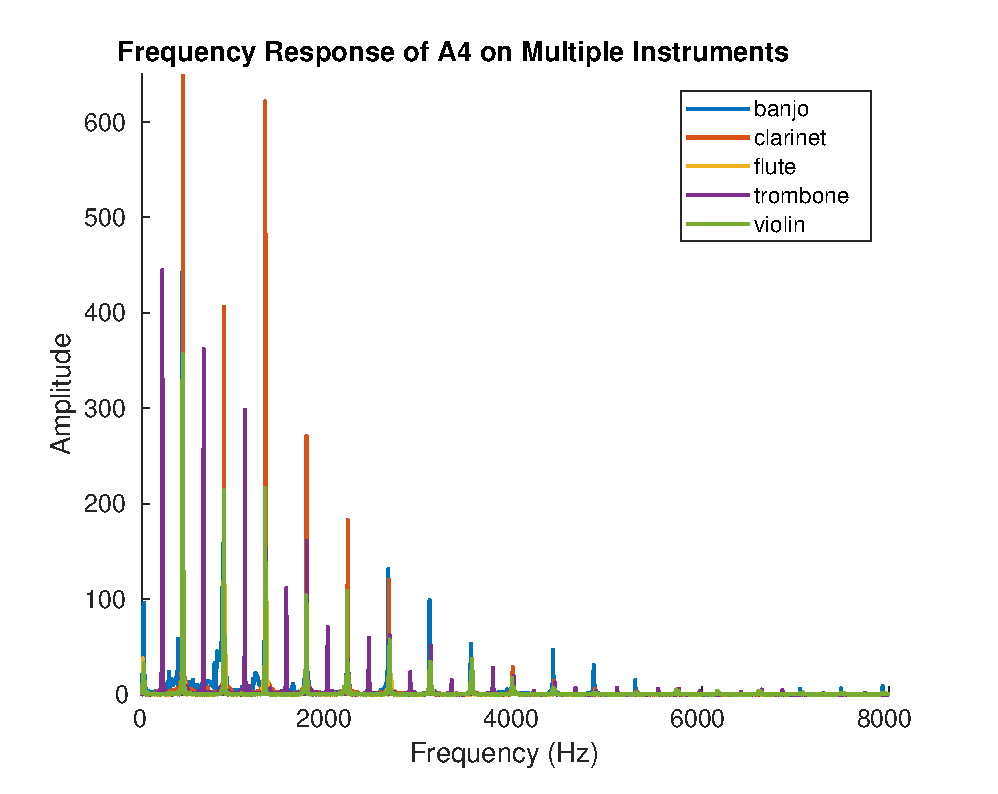
\includegraphics[width = .5\textwidth]{fft_all}
\caption{Spectra of five different instruments playing an A4 (440 Hz) tone. Variations in harmonic magnitude between instruments play a role in their characteristic sounds.}
\label{fig:fft_all}
\end{figure}

\begin{figure}[h!]
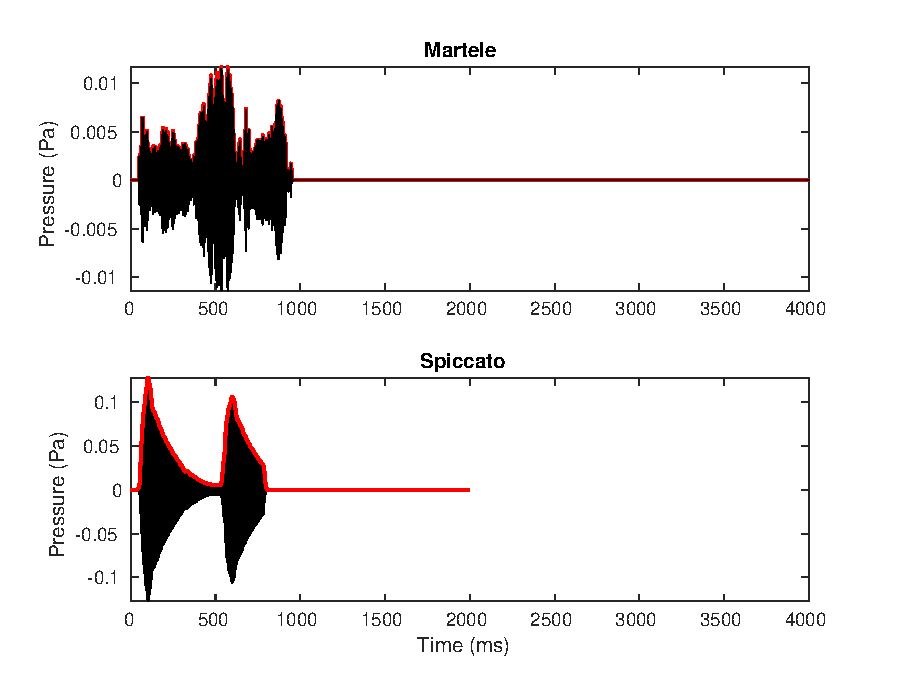
\includegraphics[width = .5\textwidth]{martele_spiccato_compare}
\caption{Variations in envelope (\textcolor{red}{red}) for two different articulations played by the violin. Waveforms were gammatone-filtered with a central frequency of 440 Hz.}
\label{fig:articulation}
\end{figure}

\subsection{The Physics of Timbre}
Variations in spectrotemporal content between instruments and their articulations is a good first step in assessing the differences in timbre from instrument to instrument. Isolating the physical characteristics of a sound played by one instrument that makes it unique from another is a key step in being able to study the coding of those characteristics. 

Figure \ref{fig:fft_all} shows the variations in the magnitude of the harmonics present in the same A4 (440 Hz) tone played on five different instruments. These same harmonics are also very pronounced in the spectrograms illustrated in Figure \ref{fig:spects}. Though it is somewhat obvious that these harmonic differences alter the physics and fine structure of a musical note, it less known how important this fine structure is in driving the coding and perception of that note by the auditory system.



The envelope of a tone also varies from instrument to instrument. Changes in envelope, even within a single instrument, can be observed by playing different articulations of that instrument. Figure \ref{fig:articulation} demonstrates variations in the envelope between the two violin articulations \textit{martel\'{e}} and \textit{spiccato}. Martel\'{e} is a more ``hammered" style of bowing, while spiccato is more ``bouncy, light, and separate."

\begin{figure*}
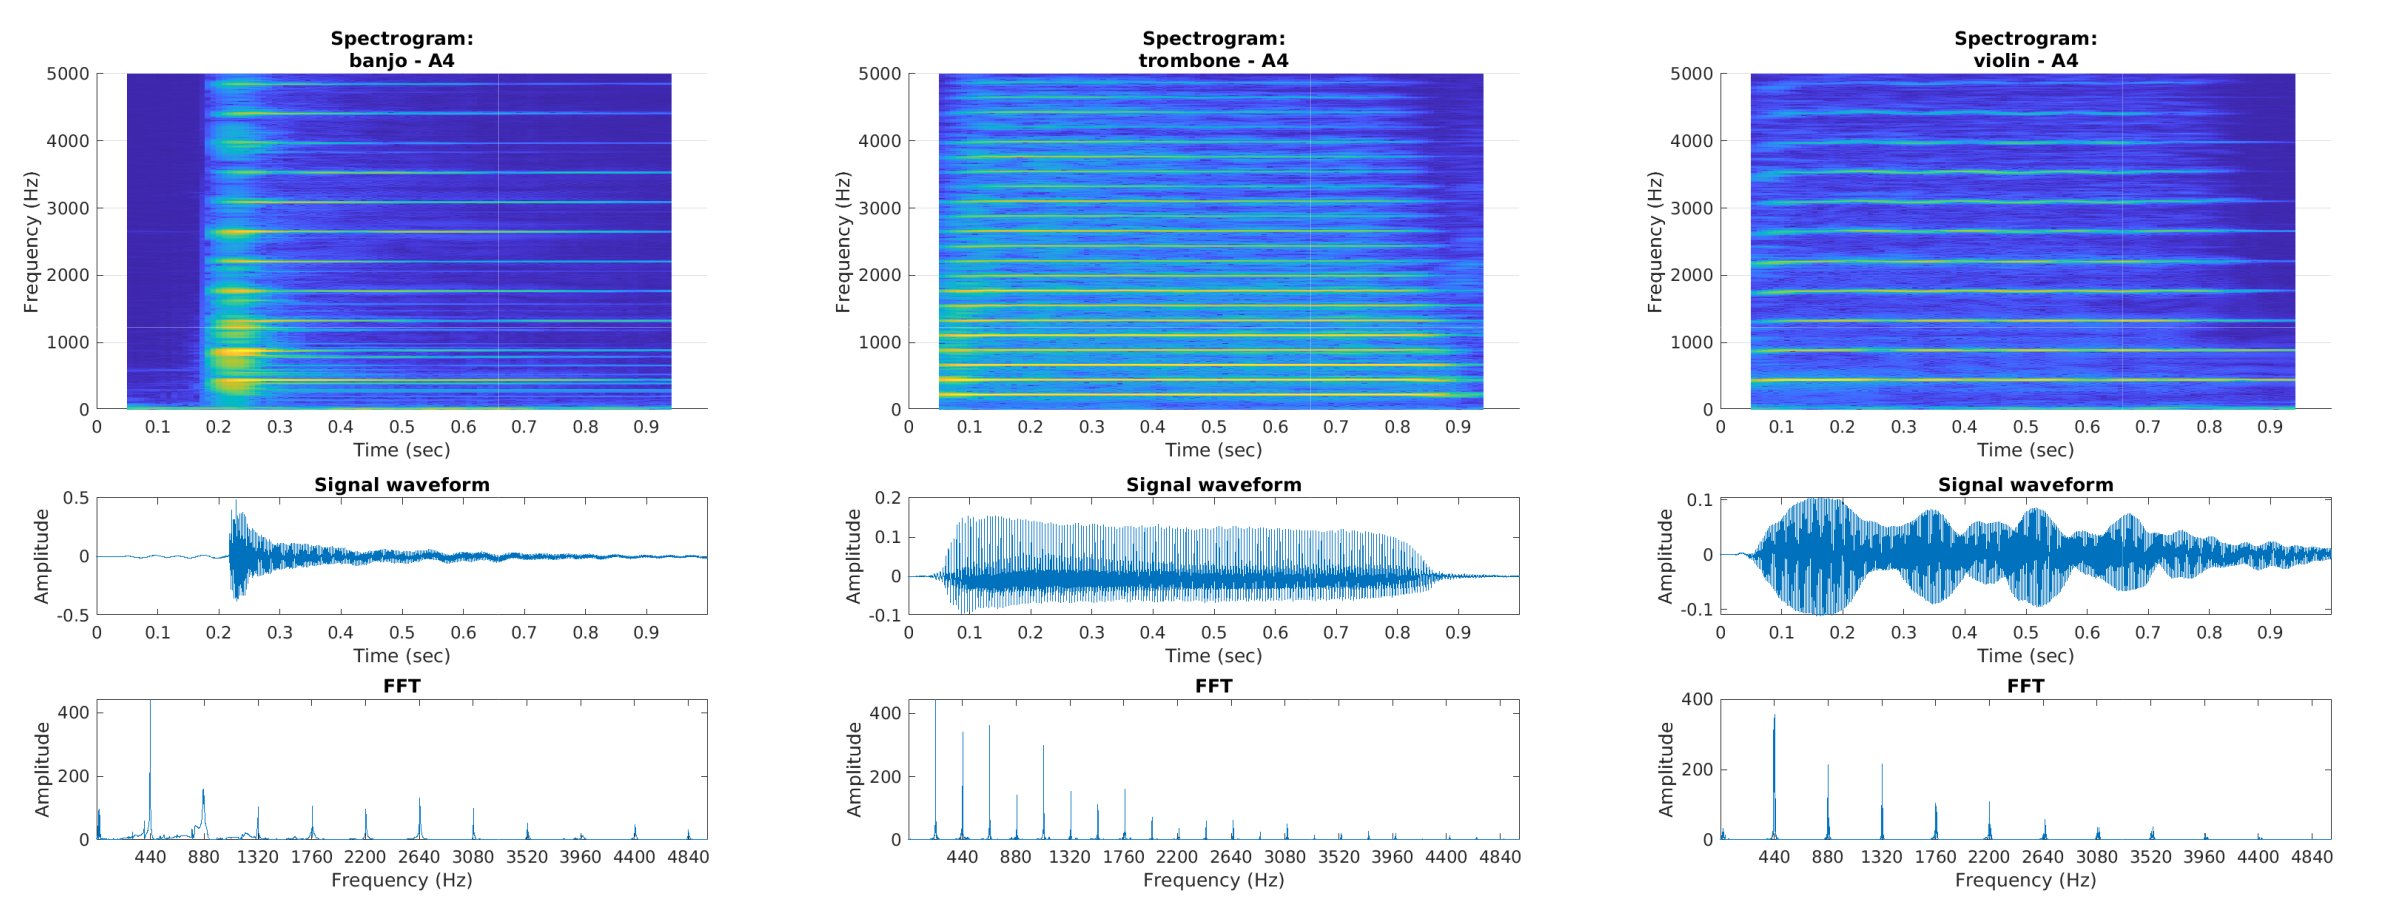
\includegraphics[width = \textwidth]{spects}
\caption{Spectrograms of three different instruments playing A4. Differences in onset and decay characterstics, modulations, and harmonic content may be visualized. Interestingly, harmonics of A3 (220 Hz) were found in the trombone recording for A4, demonstrating that timbral features may not necessarily be limited to the harmonics of the fundamental frequency of the note being played.}
\label{fig:spects}
\end{figure*}


\subsection{Methods of Analysis for Investigating TFS and ENV Neural Responses}
Much progress has been made on developing methods and analyses by which we can study how features of a particular sound stimulus reach the auditory nerve, and how they may be processed by higher order systems within the brain and brainstem. Particularly, the envelope (ENV) and temporal fine structure (TFS) of a given stimulus have been established as having relevance in its perception \cite{smith_chimaeric_2002}. However, \textit{perception }is different from \textit{coding}, and further signal processing methods were designed to characterize how TFS and ENV features are encoded by the auditory nerve \cite{heinz_quantifying_2009}. More recently, Parida et al. have developed a spectrally-specific framework for investigating ENV and TFS that can be applied to spike trains \textit{and} non-invasive far-field measures like frequency following responses (FFRs) \cite{parida_spectrally_2020}. This framework can also be applied to non-stationary signals. 

\subsection{Modeling the Auditory Nerve} 

To record neural spike data at the level of the auditory nerve is an acute and invasive process. Each experiment may span several hours, or even days.  Therefore, being sure that the stimulus presentation and signal acquistion match the question being investigated is important. One way to reduce the time needed to get data and animals needed for experimentation is using an auditory nerve model.

Zilany et al. created the auditory nerve model that was last updated in 2018, BEZ2018 \cite{bruce_phenomenological_2018}. This model is highly regarded by the field of auditory neuroscience. Though there is no replacement for true electrophysiological data, it is helpful to have an \textit{in silico} model with customizable parameters that may guide \textit{in vivo} experimentation in the future. At the very least, it allows researchers to test the validity of spike train analysis so that when \textit{in vivo} experiments may be conducted, the analysis is refined enough to answer the question at hand.
 
\subsection{A Generalizable Framework for Studying Timbre} 
 
While studies have investigated timbral \textit{perception} and have even proposed means of quantifying this perceptual ability, we are not aware of any studies that have investigated timbral \textit{coding} \cite{lee_timbre_2020}. By combining the modeling work from Zilany et al. and the spectrally specific framework designed by Parida et al., a new framework for analysis can be created to study ENV and TFS coding in various instrumental sounds and how they may or may not be impacted by hearing loss. By using this framework to identify relevant timbral coding features \textit{in silico}, recommendations for future \textit{in vivo} timbral coding experiments can be suggested. Additionally, the spectral analysis methods outlined in this new framework can be applied to \textit{both} invasive auditory nerve experiments and non-invasive FFR experiments due to the generalizabilty of the methods developed by Parida et al.
 
\section{Methods}

A framework was developed to investigate timbral coding using a combination of auditory nerve modeling and application of a spectrally-specific framework to study the strength of ENV and TFS coding across various instruments and articulations. Figure \ref{fig:flow} represents a general flow diagram of the methods used.


\subsection{Sound Stimuli}

All sound stimuli were acquired from the Philharmonia Orchestra's (UK) sound sample database \cite{noauthor_sound_nodate}. This sound sample library has thousands of neatly categorized and concise recordings that span the instrumental range of the standard orchestra, over several pitches, articulations, and expressions. The sound samples were resampled in MATLAB (Natick, MA) to 100 kHz in order to be processed by the auditory nerve model. To assess timbral coding variations between instruments, banjo, clarinet, flute, trombone, and violin A4 (440 Hz) tones were used. To assess differences in timbral coding between articulation, a martel\'{e} and spiccato sound at A4 on the violin was used. 

\subsection{Auditory Nerve Model}
The BEZ2018 model was used to generate spike histograms in response to both positive and negative polarities of the stimuli. Auditory neurons with characteristic frequencies (CFs) at 125, 440, 880, 3960 Hz were included in this simulation. In the normal hearing model, sound was played at 65 dB. The hearing-impaired condition had an average threshold shift of 43.75 dB, and this gain was added to the stimulus for a total stimulus gain of 108.75 dB. The outputs of this model were normal hearing and impaired hearing alternating-polarity peristumulus time histograms (apPSTHs) for a given stimulus, shown in Figure \ref{fig:apPSTH}. \textcolor{red}{model parameters in table?}   

\subsection{Stimulus Filtering and Hilbert Extraction}

Stimuli were passed through a computationally efficient gammatone filterbank developed by Ning Ma \cite{ma_efficient_nodate}. The center frequencies for each filter band were chosen to correspond with the auditory neuron characteristic frequentions mentioned above (125, 440, 880, 3960 Hz). The resultant channels were then processed using the Hilbert analytic signal to extract the stimulus ENV and TFS for a given CF. 

\begin{figure}
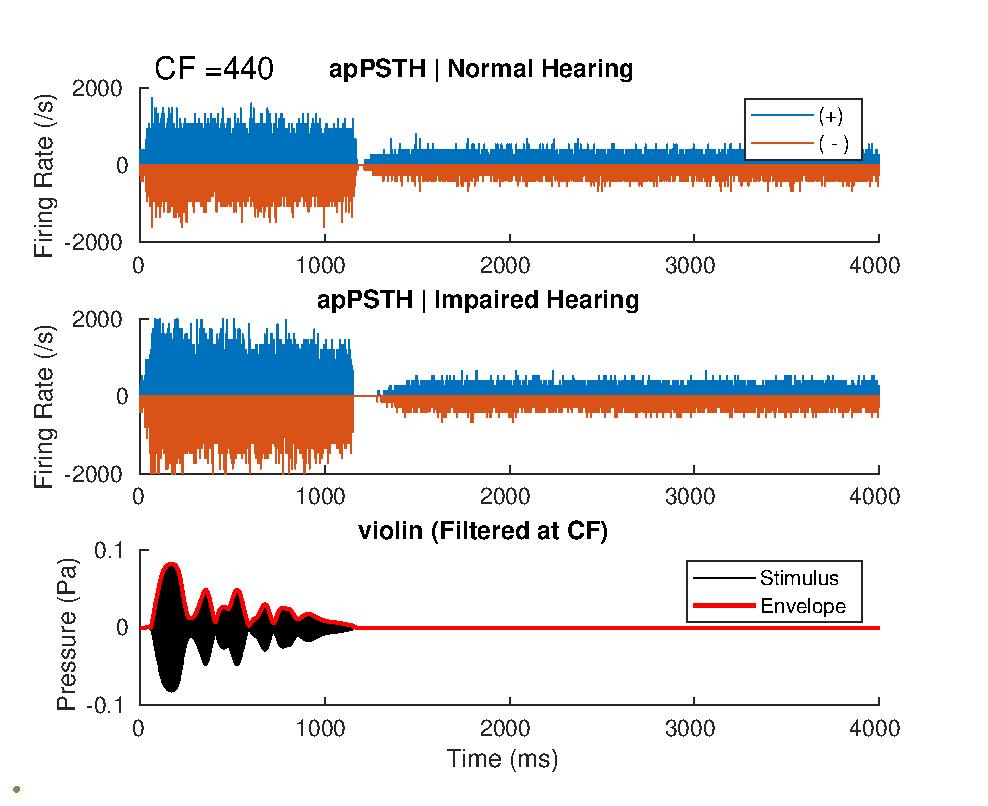
\includegraphics[width = .5\textwidth]{apPSTH_violin}
\caption{Normal and impaired hearing apPSTHs in response to a A4 on the violin filtered at CF = 440 Hz. Stimulus envelope highlighted in red in bottom figure.}
\label{fig:apPSTH}
\end{figure} 

\begin{figure*}
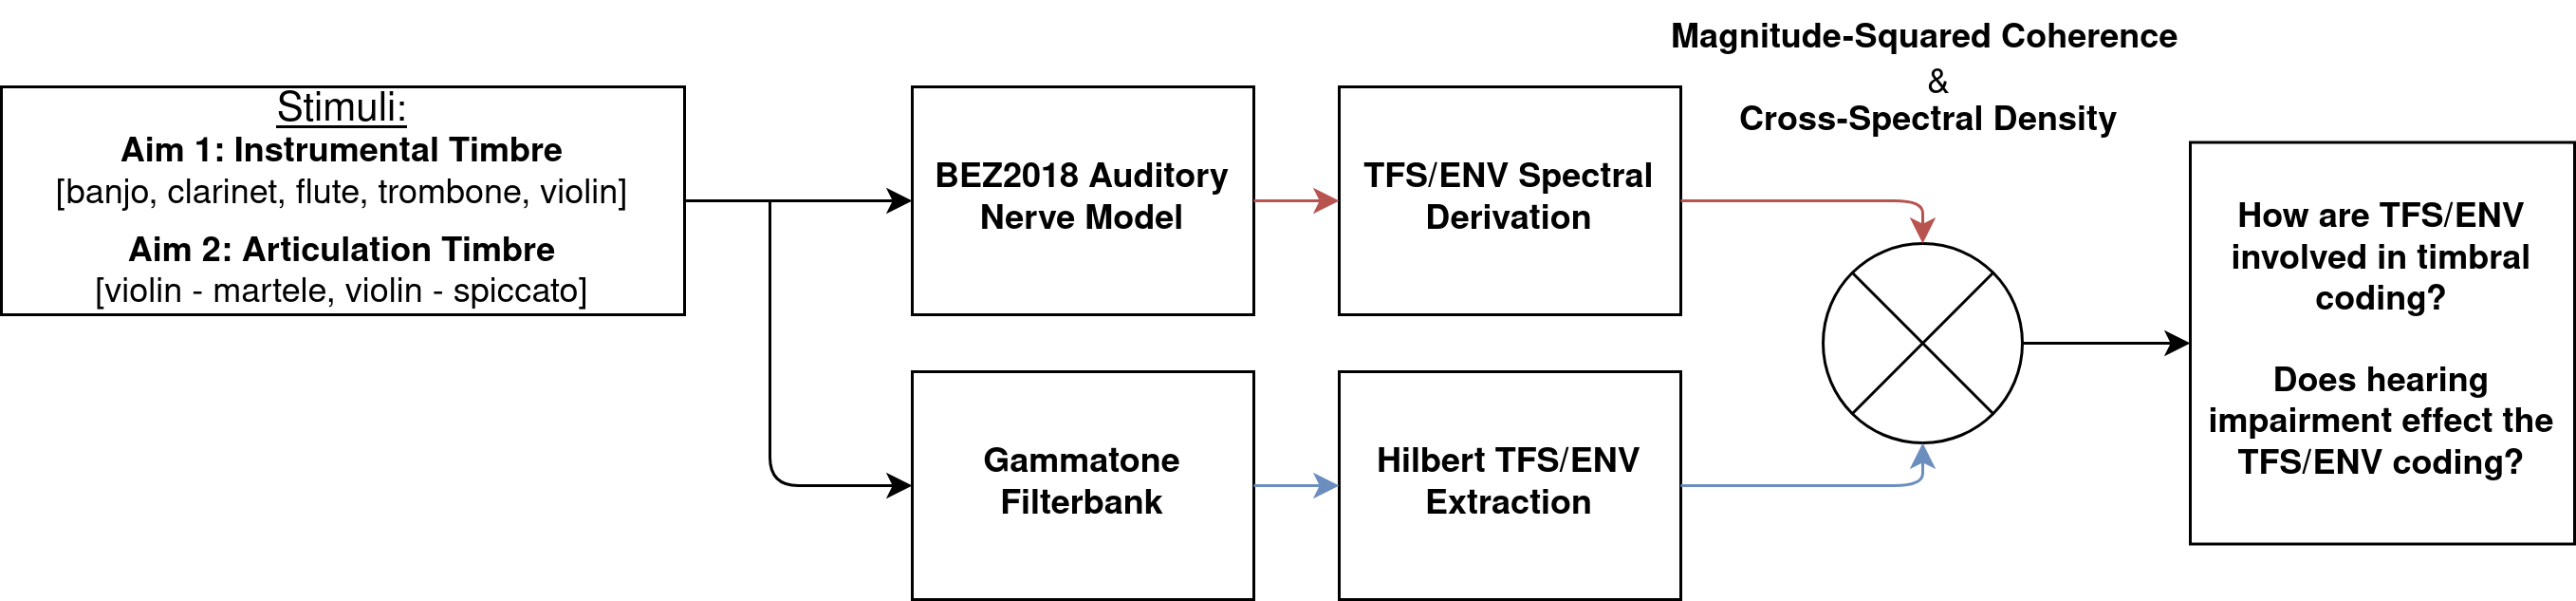
\includegraphics[width = \textwidth]{methods_flow_sanspic}
\caption{Methods flow diagram. Different instrument and articulation stimuli were processed through the BEZ2018 auditory nerve model  and through a gammatone filterbank. Alternating-polarity peristimulus time histograms (apPSTHs) (\textcolor{red}{red}) from the auditory nerve model were processed to extract TFS and ENV-related responses, and these were compared to the Hilbert TFS and ENV (\textcolor{blue}{blue}) extracted from the gammatone-filtered stimuli by means of Magnitude-Squared Coherence.}
\label{fig:flow}
\end{figure*}
\subsection{Spectral Computation and Analysis}
Using the same rationale developed by Parida et al., the ENV and TFS  response of the apPSTHs generated by the auditory nerve model were computed as $s(t)$ and $\phi(t)$, respectively:

\begin{equation}
s(t) = \frac{p(t)+n(t)}{2}
\end{equation}

\begin{equation}
d(t) = \frac{p(t)-n(t)}{2}
\end{equation}

\begin{equation}
\phi (t) = \sqrt{2} \times rms[d(t)] \times \cos[\angle d(t)]
\end{equation}

Where $p(t)$ corresponds to the positive-polarity PSTH and $n(t)$ corresponds to the negative-polarity response.

The normalized cross spectral density, magnitude-squared coherence, $C_{xy}$, was used to assess the strength of ENV and TFS coding:

\begin{equation}
C_{xy}(f) = \frac{|P_{xy}(f)^2|}{P_{xx}(f)P_{yy}(f)}
\end{equation}

Where $x$ corresponds to either $s(t)$ or $\phi(t)$ and $y$ corresponds to the Hilbert ENV or TFS of the filtered stimulus, respectively. 

\section{Results}

Magnitude-squared coherence of ENV and TFS characteristics were visually inspected in MATLAB for the different instruments and two articulations. Differences between normal and impaired hearing ENV and TFS coherence spectra were also computed. The data analysis is ongoing, but a few notable findings to date are presented here. 

\subsection{Timbral Coding of Instrumental Features}

Figure \ref{tromb_viol}  demonstrates that TFS coding of A4 in a simulated healthy auditory neuron with CF = 440 Hz played on trombone compared violin showed an additional coherence peak at approximately 490 Hz. High coherence at 440 Hz was expected in both instruments, given that there should be strong coding and phase locking of a 440 Hz tone by a neuron with CF = 440 Hz. However, a peak at 490 Hz is not a linear combination of the fundamental A4, and could be coherence related to a timbre-specific attribute present in the trombone neural response. 

\begin{figure}[h]
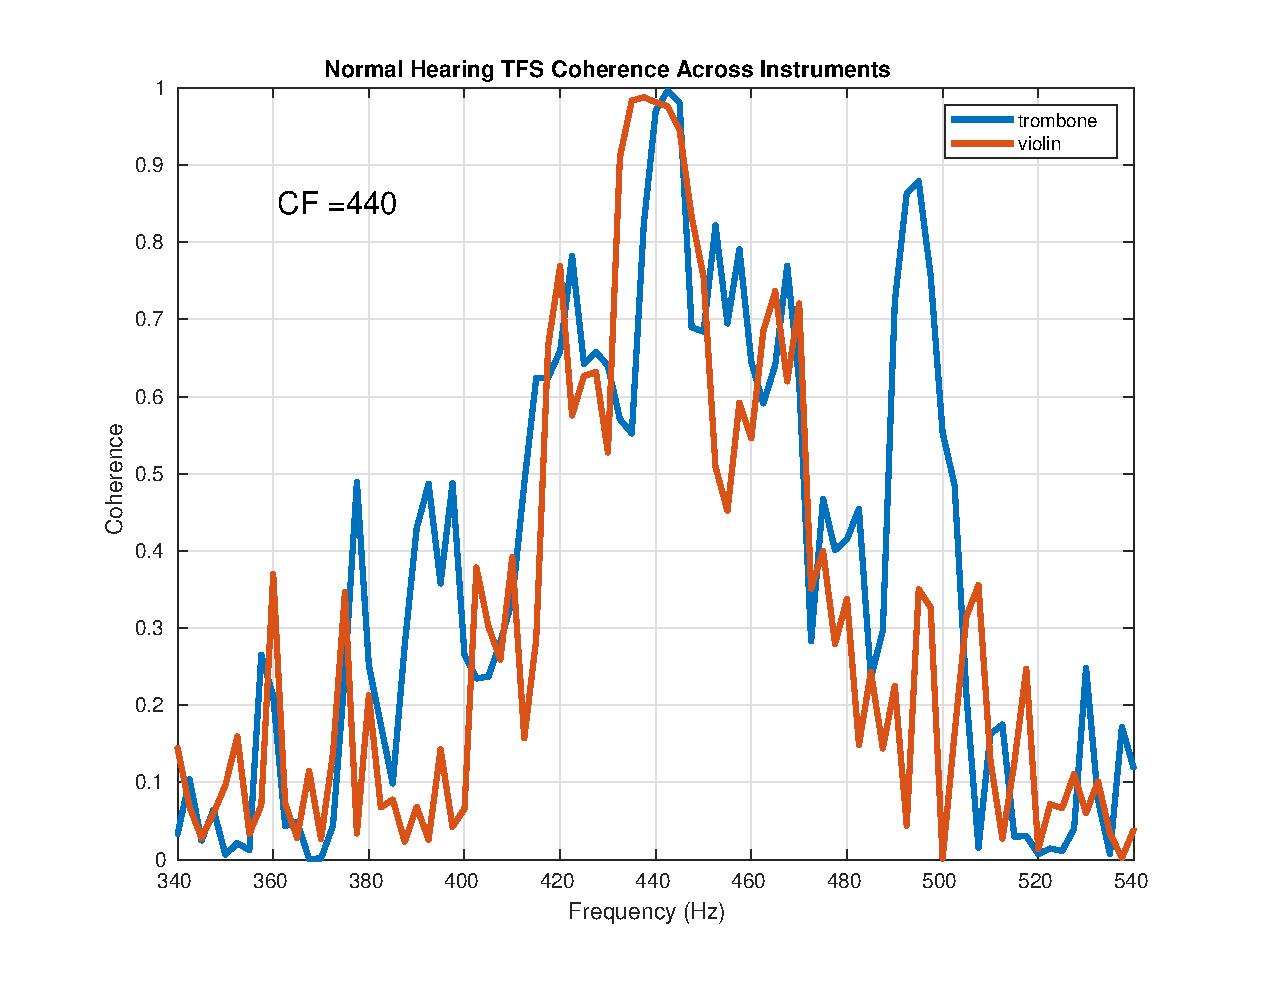
\includegraphics[width = .5\textwidth]{trombone_violin_TFS_coherence_440}
\caption{TFS coherence differences between violin and trombone in a CF = 440 Hz auditory neuron. Of particular note is a 490 Hz peak in the trombone that is absent in the violin TFS coherence.}
\label{tromb_viol}
\end{figure} 

Additionally, differences were observed in ENV coherence of violin-specific attributes in normal and impaired hearing conditions, especially in the higher-frequency neuron (CF = 3960 Hz). Figure \ref{viol_env} shows that the decreased ENV coherence in hearing impaired neurons is most pronounced in the 10-100 Hz region. 

\begin{figure}[h]
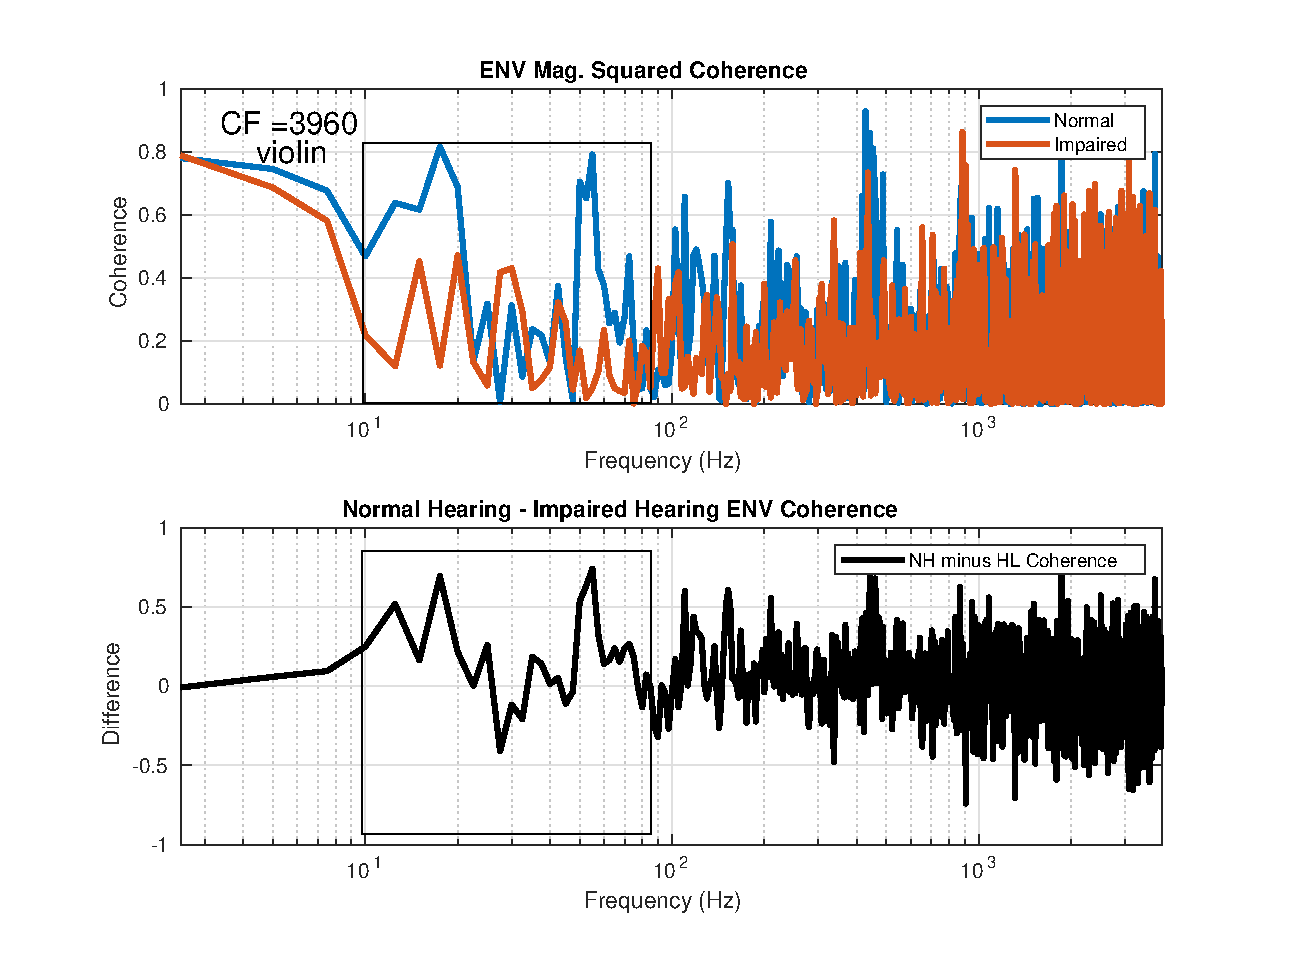
\includegraphics[width = .5\textwidth]{violin_ENV_COH_3960}
\caption{ENV coherence differences in violin A4 at CF = 3960 Hz. ENV coherence is decreased in the 10-100 Hz region (black box) in impaired neurons compared to normal hearing neurons.}
\label{viol_env}
\end{figure} 

\begin{figure}[h]
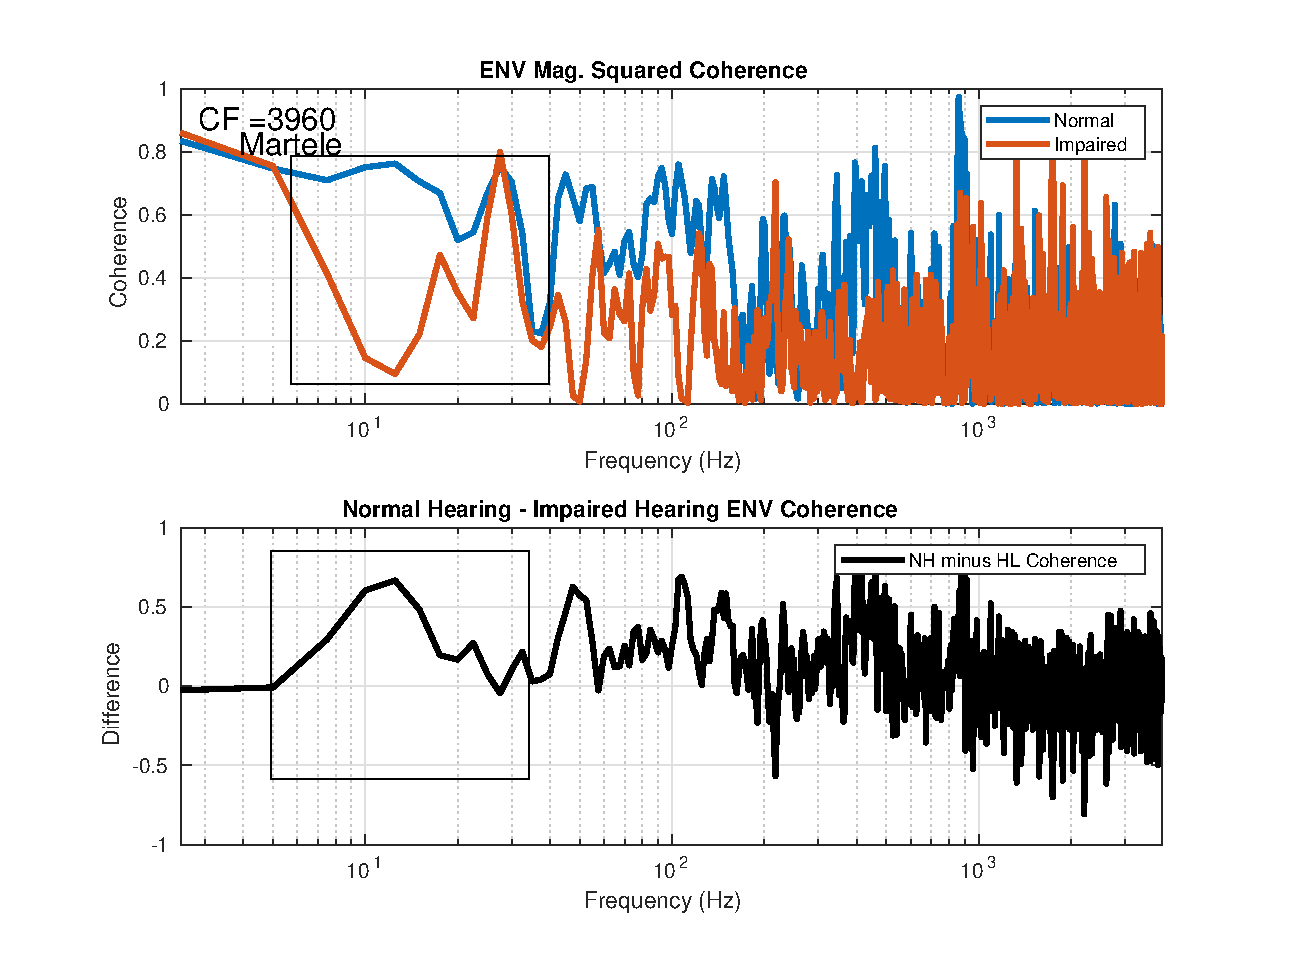
\includegraphics[width = .5\textwidth]{martele_ENV_diff}
\caption{Hearing impairment markedly decreases ENV coherence of martel\'{e} at CF = 3960 Hz. }
\label{mart_env}
\end{figure} 

\subsection{Timbral Coding of Articulation}

Martel\'{e} and spiccato also indicated differences in ENV coherence at CF = 3960. Figure \ref{mart_env} demonstrates hearing impairment particularly decreasing ENV coherence of martel\'{e} in the 6-30 Hz region. This difference in ENV coherence was not apparent in ENV coherence of spiccato at the same CF, shown in Figure \ref{spic_mart_diff}. These finding may indicate that ENV coding is particularly important in conveying timbral information related to martel\'{e}, but that this ENV coding is less important or relevant in the coding of spiccato. This may also indicate that hearing impaired listeners should more easily be able to discern ``bouncier" articulations like spiccato, as opposed to heavier articulations like martel\'{e}. 

\begin{figure}[h]
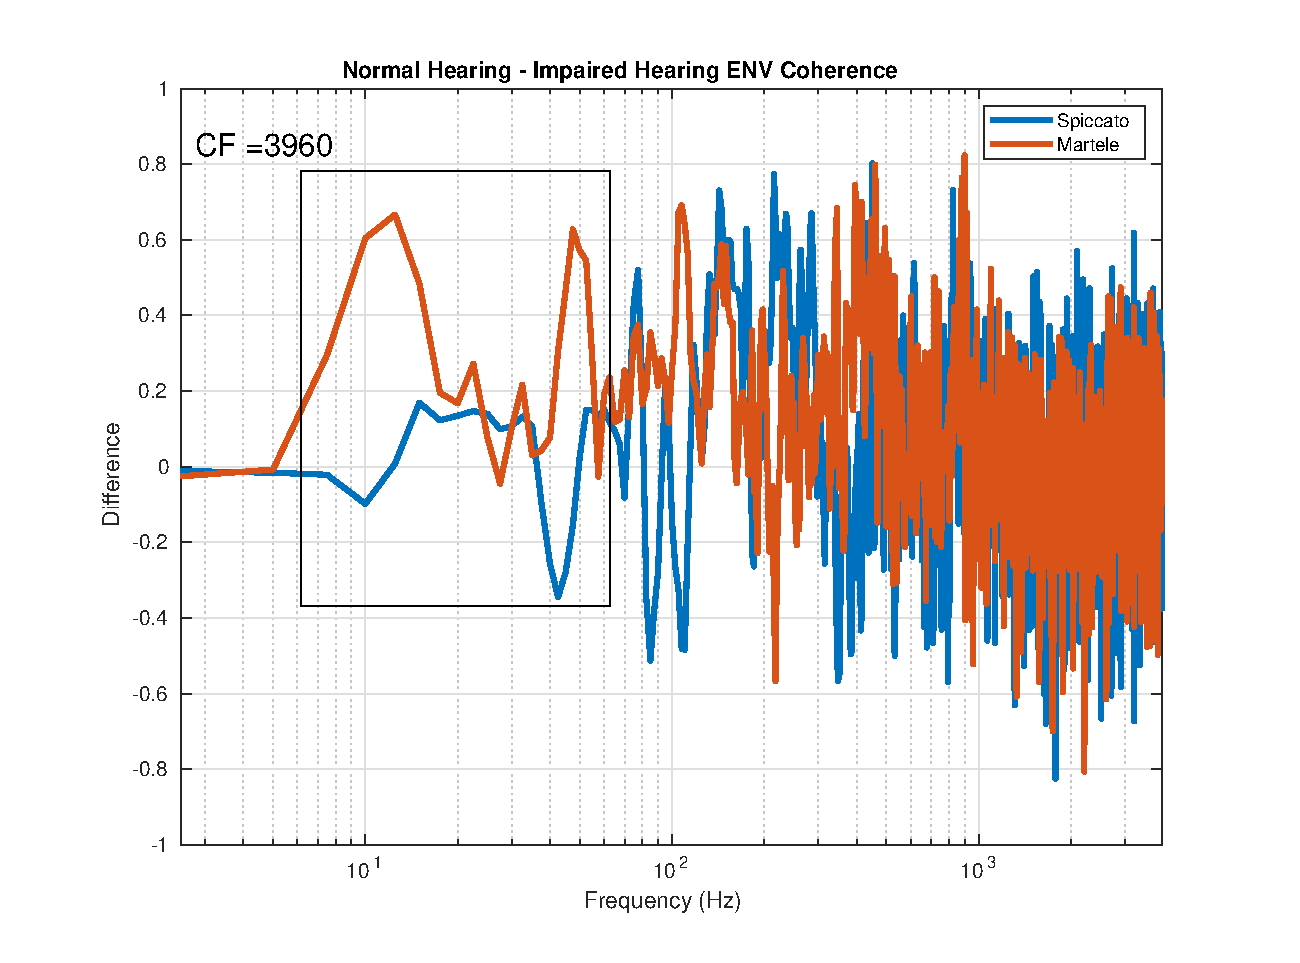
\includegraphics[width = .5\textwidth]{martele_spiccato_ENV_3960}
\caption{Hearing impairment differentially impacts martel\'{e} and spiccato ENV coherence of frequencies in the 6-30 Hz region.}
\label{spic_mart_diff}
\end{figure} 

\section{Discussion}
While this work is still preliminary, it has demonstrated the potential of using spectrally-specific measures to investigate ENV and TFS in timbral coding, while also highlighting some of the issues that may arise in future studies of timbre. 

\subsection{Coding of Timbral ENV/TFS Features} 

The data presented in this project indicate that the TFS/ENV coherence spectra vary from instrument to instrument, perhaps indicating that the auditory periphery is capable of representing and ``locking" onto timbral differences present between different instruements, even if they are playing the same tone. Additionally, the coherence spectra vary depending on the CF of the neuron. Impaired hearing may or may not result in variations in the coherence of certain timbral features, depending on the instrument or articulation being studied. 
  
\subsection{Limitations}
This project included a limited spectral analysis of the stimuli. It is evident from the uncertainty in significance or relevance present in some of the features observed in the coherence spectra. For example, it currently is unknown why a 490 Hz peak is present in the trombone coherence spectra found in Figure \ref{tromb_viol}. Additionally, it is uncertain what is resulting in the high envelope coherence in normal hearing auditory responses to the violin seen in Figure \ref{viol_env}. One may speculate that this is due to the modulation characteristics seen in the violin spectrogram shown in Figure \ref{fig:spects}. However, this speculation must be confirmed with a more thorough stimulus analysis. More closely looking at the Hilbert ENV of the stimuli or taking the spectrum of a half-wave rectification may provide more insight as to how ENV features vary from instrument to instrument before auditory processing. Another good assessment of timbral differences between instruments could be looking at timbral coherence between the stimuli themselves instead of timbral coherence of ENV and TFS between neural responses and the Hilbert ENV and TFS. 

Additionally, there are modeling parameters that should be altered in future investigation. Compensating gain for the full amount of hearing loss resulted in 108.75 dB is unrealistic and likely painful in a subject with an average of 43.75 dB hearing loss. A more realistic gain compensation would be adding half that amount or the amount needed to get a similar driven rate to the normal hearing condition. Figure \ref{fig:apPSTH} demonstrates the higher firing rate in the impaired hearing neuron, which is likely due to this unrealistic stimulus amplification.  

Finally, the spectral analysis conducted shows much variance. It is difficult to discern whether the observed coherence differences are due to variance in the estimation or whether they are part of the true coherence spectra. Because of this, it may be worth using a multi-tapered coherence spectra, similar to that conducted in a study by Viswanathan et al. \cite{viswanathan_electroencephalographic_2019}. 

\subsection{Future Study}
The framework outlined in this paper demonstrates progress towards a means of analyzing timbre coding by the auditory periphery. The analysis presented extends beyond the assessment of the BEZ2018 auditory nerve model output, and can be applied \textit{in vivo}. However, a better characterization of the timbral features present in the stimuli and a cleaner, more true, estimate of the coherence spectra are essential before progressing to such experimentation. After that, timbral coding can be better characterized and will hopefully lead to hearing aid and cochlear implant signal processing that better encapulate music features.

%\begin{table}[htbp]
%\caption{Table Type Styles}
%\begin{center}
%\begin{tabular}{|c|c|c|c|}
%\hline
%\textbf{Table}&\multicolumn{3}{|c|}{\textbf{Table Column Head}} \\
%\cline{2-4} 
%\textbf{Head} & \textbf{\textit{Table column subhead}}& \textbf{\textit{Subhead}}& \textbf{\textit{Subhead}} \\
%\hline
%copy& More table copy$^{\mathrm{a}}$& &  \\
%\hline
%\multicolumn{4}{l}{$^{\mathrm{a}}$Sample of a Table footnote.}
%\end{tabular}
%\label{tab1}
%\end{center}
%\end{table}
%
%\begin{figure}[htbp]
%\centerline{\includegraphics{fig1.png}}
%\caption{Example of a figure caption.}
%\label{fig}
%\end{figure}


\section*{Acknowledgment}

Without my family, music instructors, and teachers I would not have been so motivated to study the relevance of music in auditory neuroscience. Additionally, without the support and wisdom from Dr. Satya Parida (and however many coconuts he has sacrificed to the Gods of auditory neuroscience), this project would have been much more challenging. Finally, the feedback received by the Heinz Lab on Tuesday has made it clearer what the next steps in this project should be.

%\section*{References}


\bibliographystyle{ieeetr}
%laptop
%\bibliographystyle{IEEEtran} 

\bibliography{references}{}

\end{document}
